
%%%%%%%%%%%%%%%%%%%%%%%%%%%%%%%%%%%%%%%%%%%%%%%%%%%%%%%%%%
\chapter{Conclusions and Future Work}
\label{chapter_conclusions_and_future_work}
%%%%%%%%%%%%%%%%%%%%%%%%%%%%%%%%%%%%%%%%%%%%%%%%%%%%%%%%%%

\section{Conclusions}

\newtext
{
We presented three deformation-driven packing methods.
FLOWPAK is a method to deform and pack long thin elements to follow a vector field.
RepulsionPak is a method that uses repulsion forces to pack and deform
elements that are represented as mass-spring systems.
AnimationPak is an extension of RepulsionPak that packs animated 2D elements,
each an extruded 3D shape in a spacetime domain.
}

\newtext
{
Given a small size element library, 
we demonstrated that deformation-driven methods can create element compatibilities
and fill the container effectively.
Repeated elements give a sense of uniformity but deformation creates a sense of variety.
%As element compatibilities are increased, the negative space is more even.
}

\newtext
{
We discussed the evenness of negative space as an indicator of the quality of a packing.
We measured the evenness using three statistical metrics:
spherical contact probabilities, histograms of distance transforms, and overlap functions.
}

\section{Future Work}

\newtext
{
This thesis in only the tip of the iceberg of packing research as
we see many possibilities for future work.
}


%%%%%%%%%%%%%%%%%%%%%%%%%%%%%%%%%%%%%%%%%%%%%%%%%%%%%%%%%%%%%%%%%%%%%%%%%%%%%%%%%%%%%%%%%%
%%%%%%%%%%%%%%%%%%%%%%%%%%%%%%%%%%%%%%%%%%%%%%%%%%%%%%%%%%%%%%%%%%%%%%%%%%%%%%%%%%%%%%%%%%
%%%%%%%%%%%%%%%%%%%%%%%%%%%%%%%%%%%%%%%%%%%%%%%%%%%%%%%%%%%%%%%%%%%%%%%%%%%%%%%%%%%%%%%%%%
\subsection{Element Manufacturing}

\nnewtext{Unlike data-driven methods and deformation-driven methods,
we would like to manufacture a new element on the fly during the packing process.
A simple example is demonstrated in a FLOWPAK result (Figure~\ref{result_bear_offset}), 
where new elements are created from the unused negative space.
A manufactured element is also useful to create a fixed element (Chapter~\ref{chapter_flowpak}).}
This can be done perhaps by discovering them as salient regions 
in source photographs, and extracting and vectorizing them.  This 
extraction must be carried out carefully, yielding enough fixed elements
to communicate a container clearly without disrupting the uniformity of
the design.

\nnewtext{Another idea is to manufacture \textit{modular} elements assembled from smaller subparts.
A modular element can increase its compatibility by swapping its subparts.
We would like to investigate several shape synthesis methods by 
Baxter and Anjyo~\cite{Baxter2006},
Risser et al.~\cite{Risser2010}, Kalogerakis et al.~\cite{Kalogerakis2012}, 
and Hurtut and Landes~\cite{Hurtut2012}. 
Data-driven methods can benefit from this approach as we are able to 
generate large combinations of elements from a collection of subparts.
We can also work toward uniformity amidst variety principle 
as we can generate similar elements with varying subparts.
}

\begin{figure}
\centering
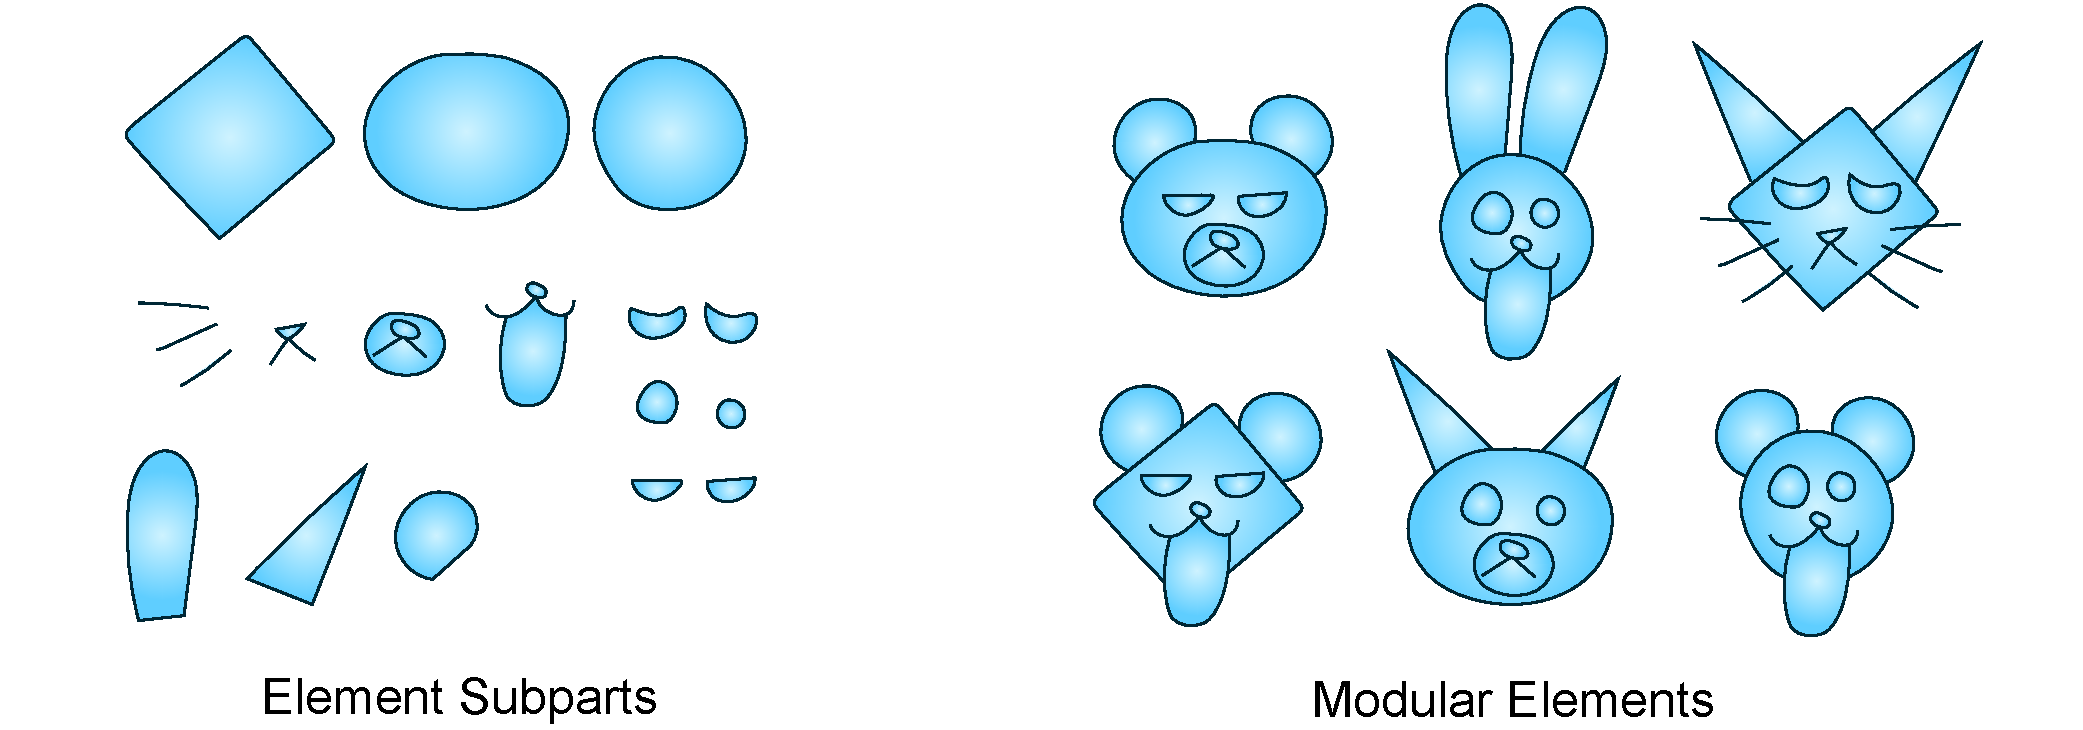
\includegraphics[width=1.0\textwidth]{figures/conclusions/modular.pdf}
\caption[Modular elements]
{ \label{modular_element} 
\nnewtext
{
Examples modular elements assembled from smaller parts to create element compatibilities.
}
}
\end{figure}

\nnewtext{We also consider an idea of plant-style modular elements.
In Figure~\ref{thread_branch}a, we can
combine multiple shorter elements
by threading them on a curve to create a longer modular element.
In Figure~\ref{thread_branch}b, we can also
try to generate branching structures to resemble floral ornaments.
In both instances, there are several challenges we have to face.
First, we need a way to connect the overlapping segments of the elements together
to create smooth and plausible transitions.
An ornament synthesis method such as DecoBrush~\cite{Lu2014} may be worth investigating.
This leads us to a deeper research topic:
how to develop a content-aware blending method on vector graphics patterns.
Second, we also should consider the semantics of the element shapes.
Not every part of an element can be connected; for example, a twig
cannot be attached onto the tip of a leaf.}

\nnewtext{
Modular elements give us opportunities to perform a smarter element placement.
The first idea is similar to JIM method,
but we are able to backtrack to previous arrangements 
that have not only different elements but also different parts.
The second idea is to perform partial shape matching only between salient container features and
element subparts. Once a matching subpart is attached to a salient feature, we can then manufacture an entire
element based on that subpart.}





\begin{figure}
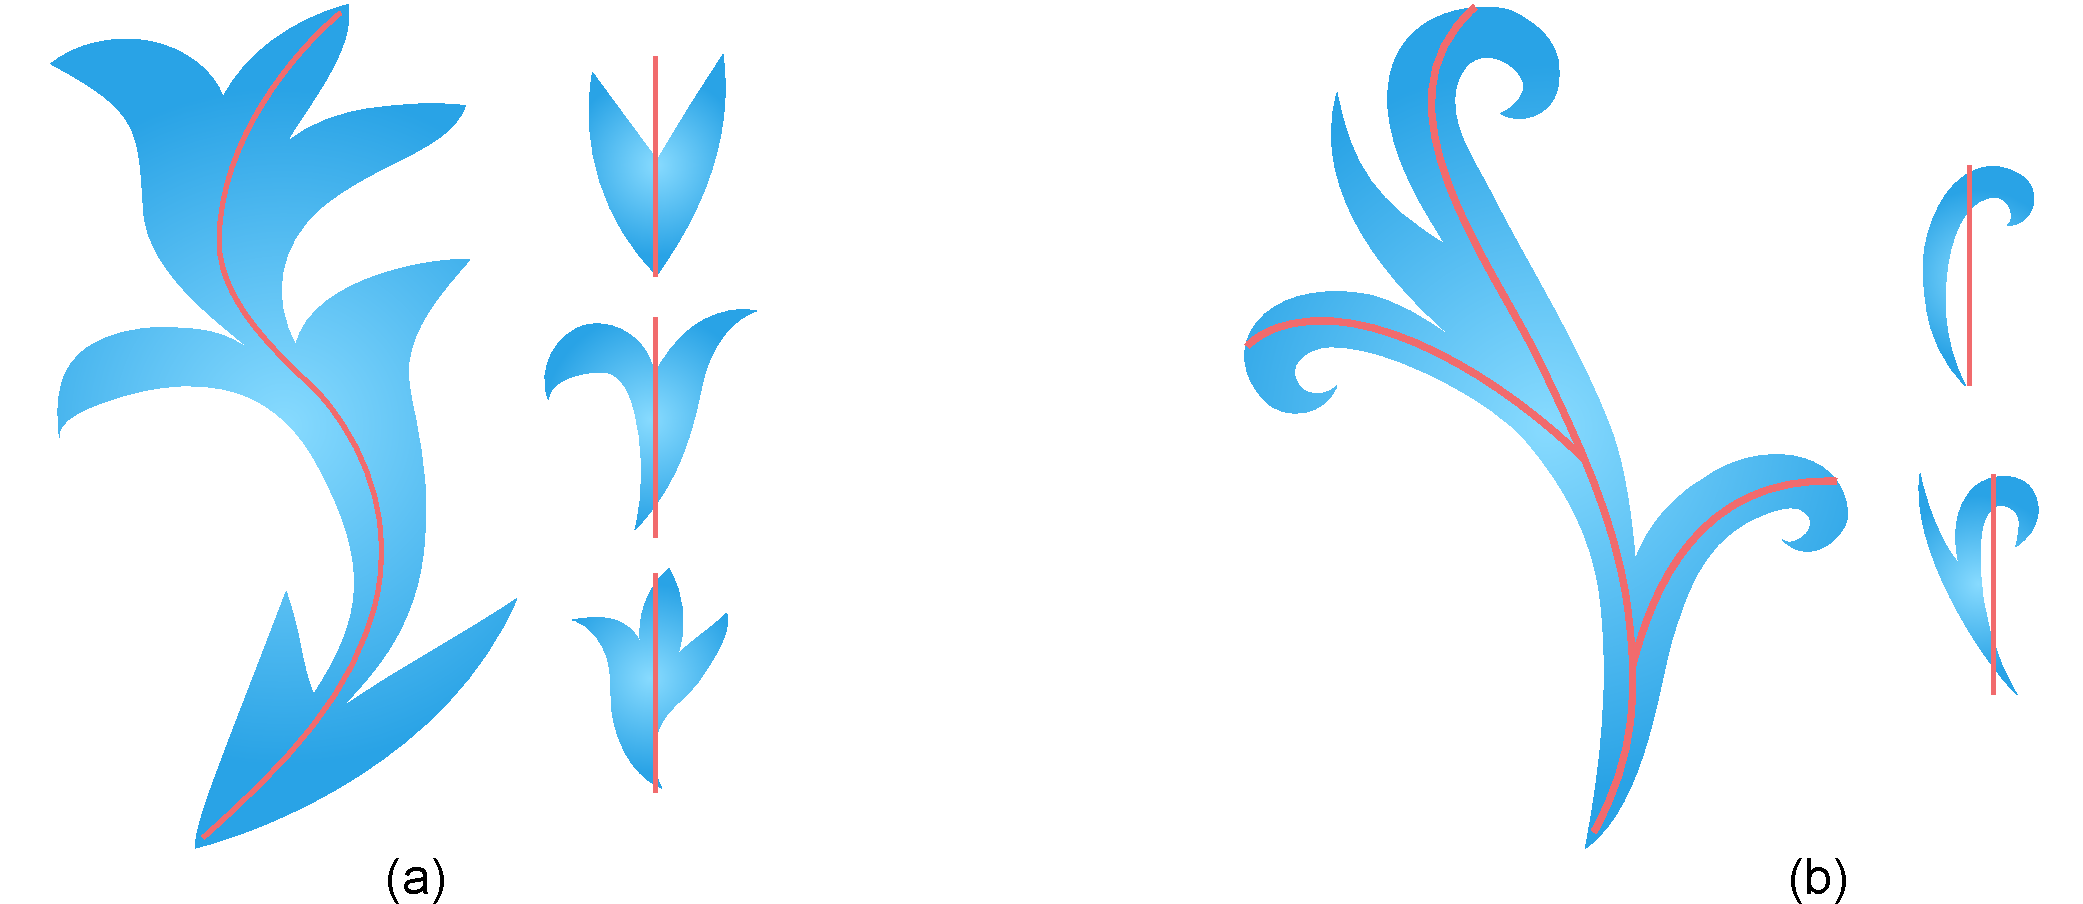
\includegraphics[width=1.0\textwidth]{figures/conclusions/thread_branch_3.pdf}
\caption[Element threading and branching]
{ \label{thread_branch} 
\nnewtext
{
Plant-style modular elements.
(a) Thread multiple elements to create a longer element.
(b) Combine multiple streamlines to create branching.
}
}
\end{figure}


%%%%%%%%%%%%%%%%%%%%%%%%%%%%%%%%%%%%%%%%%%%%%%%%%%%%%%%%%%%%%%%%%%%%%%%%%%%%%%%%%%%%%%%%%%
%%%%%%%%%%%%%%%%%%%%%%%%%%%%%%%%%%%%%%%%%%%%%%%%%%%%%%%%%%%%%%%%%%%%%%%%%%%%%%%%%%%%%%%%%%
%%%%%%%%%%%%%%%%%%%%%%%%%%%%%%%%%%%%%%%%%%%%%%%%%%%%%%%%%%%%%%%%%%%%%%%%%%%%%%%%%%%%%%%%%%
\subsection{Collaborations with Artists}

\nnewtext{
We believe that collaborations with artists can provide us invaluable feedback for our deformation-driven methods.
Two artists have used RepulsionPak to generate packing in Figure~\ref{paul_daichi_packings},
although we did not have the chance to ask for their feedback.
We also receive interests from online communities to use RepulsionPak for graphic design applications.}

\nnewtext{We would like to develop} an interactive user interfaces for our packing methods.
Examples of recent work in this style include research
by Zehnder et al.~\cite{Zehnder2016}, Gieseke et al.~\cite{Gieseke2017}, 
and Hsu et al.~\cite{Hsu2020}, which let the user directly place and manipulate
elements while a composition is being created.
\nnewtext{
Inspired by doodle murals by Joe Whale (Figure~\ref{doodle_boy}), 
it would be interesting to display an interactive packing on a large touch screen,
and let artist to draw elements, which are then rearranged using RepulsionPak.
}

\nnewtext{In the context of animated packings,} 
we were only able to find a single example from The Simpsons (Figure~\ref{fig_animationpak_lisa_packing}). 
We think its unpopularity is because it is difficult and time-consuming to create by hand.
Therefore, we would like to engage with artists to understand the aesthetic value and limitations
of AnimationPak.


\begin{figure}
\centering
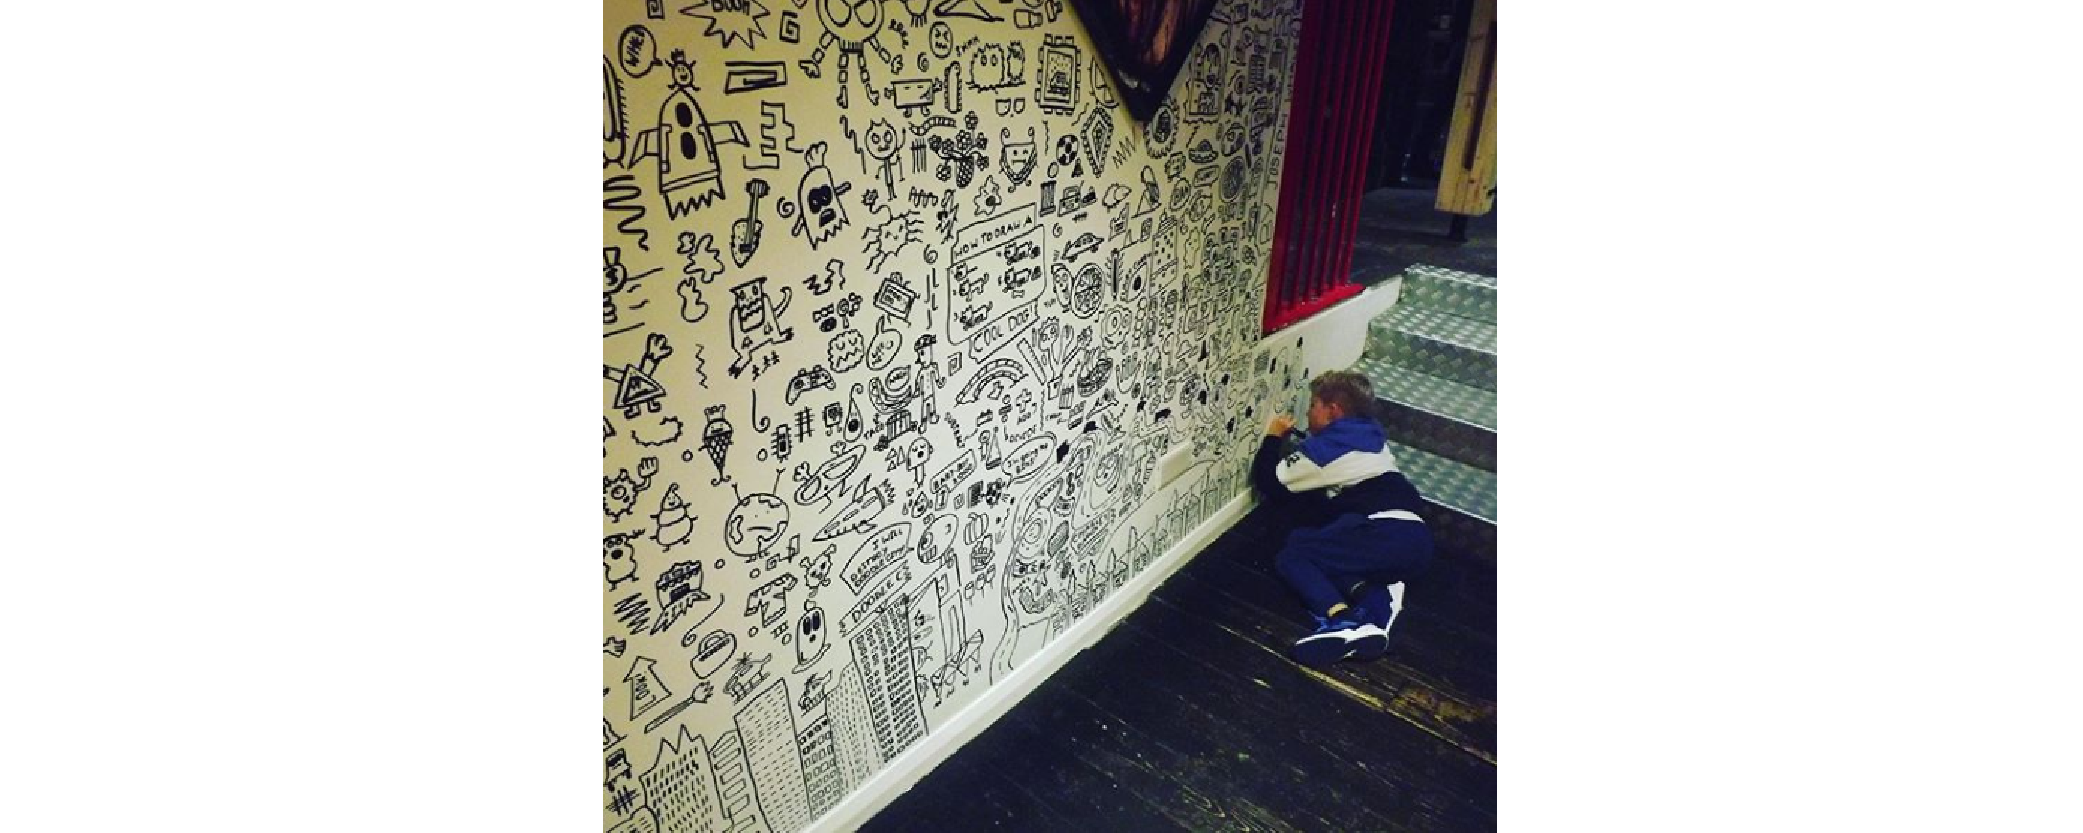
\includegraphics[width=1.0\textwidth]{figures/conclusions/doodle_boy.pdf}
\caption[A doodle mural by Joe Whale]
{ \label{doodle_boy} 
\nnewtext
{
A young artist, Joe Whale, is drawing a doodle mural. 
The photograph is taken from instagram.com/thedoodleboy.co.uk.
}
}
\end{figure}


%%%%%%%%%%%%%%%%%%%%%%%%%%%%%%%%%%%%%%%%%%%%%%%%%%%%%%%%%%%%%%%%%%%%%%%%%%%%%%%%%%%%%%%%%%
%%%%%%%%%%%%%%%%%%%%%%%%%%%%%%%%%%%%%%%%%%%%%%%%%%%%%%%%%%%%%%%%%%%%%%%%%%%%%%%%%%%%%%%%%%
%%%%%%%%%%%%%%%%%%%%%%%%%%%%%%%%%%%%%%%%%%%%%%%%%%%%%%%%%%%%%%%%%%%%%%%%%%%%%%%%%%%%%%%%%%
\subsection{Beyond 2D}

\nnewtext{We would like to explore the use of deformation-driven methods in a fabrication context.
Specifically, we want to pack 2D elements on surfaces.
For example, our boundary compatibilities might be used to create a connected object.
Alternatively, it would be interesting to 3D print the 
negative space, which is already connected due to the absence of overlaps.
The resulting packing is the shape of negative space with holes from element shapes.}

\nnewtext{Many of the techniques in this thesis could be adapted
to develop a deformation-driven method for packing purely spatial
3D objects in a 3D container.  
We would like to evaluate the
expressivity and visual quality of deformation-driven 3D packings 
in comparison to other 3D packing techniques.
One potential issue is that elements in the middle may be fully occluded by their neighbors,
which would render them useless as they cannot be viewed.
This problem will arise especially in a dense 3D packing of small elements.}

\nnewtext{Another interesting idea would be generating a bas-reliefs using a packing method,
which can be called as a 2.5D packing.
Figure~\ref{borobudur} shows a two bas-reliefs from Borobudur temple, Indonesia,
each relief consists of tight arrangement of human shapes although it does not 
have interlocking style of packings.
We see this problem as arranging non-overlapping 3D elements on surfaces, 
which include not only 2D panels but also any 3D surfaces.
Each 3D element can still rotate in all three axes but still attached to the surface.
As seen in the Borobudur reliefs, elements may occlude but they do not actually overlap,
it would be interesting to investigate aesthetics value of 2.5D packings that allow some amount of occlusions
as the consequence of 3D rotations but are still overlaps free.
%This rotation freedom leads to another interesting question: can we allow slight occlusions
%but the the elements are still overlap-free as seen in the Borobudur reliefs?
}
%Unlike a standard 3D packing, we can avoid fully occluded elements.



\begin{figure}
\centering
\includegraphics[width=1.0\textwidth]{figures/conclusions/borobudur.pdf}
\caption[Element Arrangements in Bas-Reliefs]
{ \label{borobudur} 
\nnewtext
{
Bas-reliefs from Borobudur temple. These
bas-reliefs give us an idea to generate a packing of 3D objects on a 2D panel,
or we call it as a 2.5D packing.
Individual element can still rotate in 3D to align itself with its neighbors.
The photographer of the left image was Michael Gunther, and the right image was taken by Michel Estermann.
}
}
\end{figure}

%%%%%%%%%%%%%%%%%%%%%%%%%%%%%%%%%%%%%%%%%%%%%%%%%%%%%%%%%%%%%%%%%%%%%%%%%%%%%%%%%%%%%%%%%%
%%%%%%%%%%%%%%%%%%%%%%%%%%%%%%%%%%%%%%%%%%%%%%%%%%%%%%%%%%%%%%%%%%%%%%%%%%%%%%%%%%%%%%%%%%
%%%%%%%%%%%%%%%%%%%%%%%%%%%%%%%%%%%%%%%%%%%%%%%%%%%%%%%%%%%%%%%%%%%%%%%%%%%%%%%%%%%%%%%%%%
\subsection{Packing Evaluation}

We would like to develop additional metrics to evaluate
how well an ornamental design fulfills other design principles.
\newtext{In Chapter~\ref{chapter_flowpak}, we argue that visual flow and
``uniformity amidst variety'' are important in attractive packings.} 
In another study, Wong et al.~\cite{Wong1998} describe basic design
principles for decorative arts: repetition, balance, and conformation
to geometric constraints. 

A measure of element deformation in a composition would permit 
a comparison against future deformation-driven techniques.
In RepulsionPak, we can measure the potential energy at equilibrium.
However, there are some questions to answer.
Can we measure how deformations are perceived? How much they affect the aesthetics of packings?
Such measurements could help us develop better deformation algorithms in generally, not just in the context of packings.
%Can we measure how much deformation has happened (RepulsionPak: measure the potential energy left in the system at equilibrium?).  Can we measure how easily deformations are perceived, how much they affect the aesthetics of packings? In the long run, such measurements could help us develop better deformation algorithms more generally, not just in the context of packings.

All three metrics described in Chapter~\ref{chapter_qualitative_metrics} are only for evaluating 2D packings.
While they extend naturally to three purely spatial dimensions, 
it is not clear whether they can be adapted to the spacetime context.  
We would like to investigate spatial statistics for the quality of animated packings created by AnimationPak that correlate
with human perceptual judgments.

